\section{実験結果}

\subsection{ビッカース硬さ試験}
表\ref{tbl:ビッカース硬さ結果}にビッカース硬さの測定結果,表\ref{tbl:ビッカース硬さ平均}にビッカース硬さの平均と標準偏差を示す.

\begin{table}[htbp]
    \centering
    \caption{Vickers hardness test results.}
    \label{tbl:ビッカース硬さ結果}
    \scalebox{0.7}{
    \begin{tabular}{ccccc}
    \hline
    試験回数 & 対角線長さ(横){[}$\mathrm{\mu m}${]} & 対角線長さ(縦){[}$\mathrm{\mu m}${]} & 対角線長さの平均値{[}$\mathrm{\mu m}${]} & ビッカース硬さ$\mathrm{H_v}${[}GPa{]} \\ \hline
    1    & 157.3            & 154.0            & 155.65            & 0.74995            \\ \hline
    2    & 156.0            & 157.8            & 156.90            & 0.73805            \\ \hline
    3    & 157.2            & 154.6            & 155.90            & 0.74755            \\ \hline
    4    & 157.2            & 155.1            & 156.15            & 0.74516            \\ \hline
    5    & 158.4            & 159.2            & 158.80            & 0.72050            \\ \hline
    \end{tabular}
    }
\end{table}

\begin{table}[htbp]
    \centering
    \caption{Mean and standard deviation of Vickers hardness.}
    \label{tbl:ビッカース硬さ平均}
    \scalebox{0.8}{
    \begin{tabular}{ccc}
    \hline
                       & 平均値$\mathrm{H_v}${[}GPa{]} & 標準偏差{[}GPa{]} \\ \hline
    ビッカース硬さ$\mathrm{H_v}${[}GPa{]} & 0.7402         & 0.01190       \\ \hline
    \end{tabular}
    }
\end{table}

\subsection{摩擦試験}

摩擦係数の測定結果をボール試験片の曲率半径$R$ = 1mm,4mm,8mmのそれぞれについて表\ref{tbl:ボール半径1}から表\ref{tbl:ボール半径8}にかけて示す.また,横軸に摩擦係数の平均値$\mu$,縦軸に垂直荷重$W$として測定結果をプロットしたものを図\ref{fig:fig_1mm}から図\ref{fig:fig_8mm}にかけてそれぞれ示す.

どの曲率半径においても,垂直荷重の増加による摩擦係数の変化はほとんど起こっていない.$R$ = 1mmと4mmを比較しても,摩擦係数の変化はほとんど見られない.$R$ = 8mmの場合は,垂直荷重が小さいため,相対的に外乱の影響が大きくなっており,標準偏差が大きくなっている.

\begin{table}[htbp]
    \centering
    \caption{Coefficient of friction measurement results(R=1[mm]).}
    \label{tbl:ボール半径1}
    \scalebox{1.0}{
    \begin{tabular}{cccc}
    \hline
    試験回数 & 0.98{[}N{]} & 4.9{[}N{]} & 9.8{[}N{]} \\ \hline
    1    & 0.676       & 0.673      & 0.656      \\ \hline
    2    & 0.635       & 0.614      & 0.622      \\ \hline
    3    & 0.621       & 0.569      & 0.658      \\ \hline
    4    & 0.564       & 0.56       & 0.71       \\ \hline
    5    & 0.56        & 0.604      & 0.744      \\ \hline
    平均値μ & 0.611       & 0.604      & 0.678      \\ \hline
    標準偏差 & 0.0493      & 0.0448     & 0.0485     \\ \hline
    \end{tabular}
    }
\end{table}
\begin{table}[htbp]
    \centering
    \caption{Coefficient of friction measurement results(R=4[mm]).}
    \label{tbl:ボール半径4}
    \scalebox{1.0}{
    \begin{tabular}{cccc}
    \hline
    試験回数 & 0.98{[}N{]} & 4.9{[}N{]} & 9.8{[}N{]} \\ \hline
    1    & 0.581       & 0.601      & 0.585      \\ \hline
    2    & 0.546       & 0.53       & 0.566      \\ \hline
    3    & 0.557       & 0.495      & 0.625      \\ \hline
    4    & 0.638       & 0.492      & 0.69       \\ \hline
    5    & 0.612       & 0.54       & 0.568      \\ \hline
    平均値μ & 0.587       & 0.532      & 0.607      \\ \hline
    標準偏差 & 0.0382      & 0.0442     & 0.0522     \\ \hline
    \end{tabular}
    }
\end{table}
\begin{table}[htbp]
    \centering
    \caption{Coefficient of friction measurement results(R=8[mm]).}
    \label{tbl:ボール半径8}
    \scalebox{1.0}{
    \begin{tabular}{cccc}
    \hline
    試験回数 & 0.098{[}N{]} & 0.196{[}N{]} & 0.49{[}N{]} \\ \hline
    1    & 0.839        & 0.417        & 0.61        \\ \hline
    2    & 0.454        & 0.418        & 0.61        \\ \hline
    3    & 0.656        & 0.657        & 0.572       \\ \hline
    4    & 0.718        & 0.639        & 0.613       \\ \hline
    5    & 0.558        & 0.693        & 0.542       \\ \hline
    平均値μ & 0.645        & 0.565        & 0.589       \\ \hline
    標準偏差 & 0.148        & 0.136        & 0.0314      \\ \hline
    \end{tabular}
    }
\end{table}

\begin{figure}[htbp]
    \centering %中央揃え
    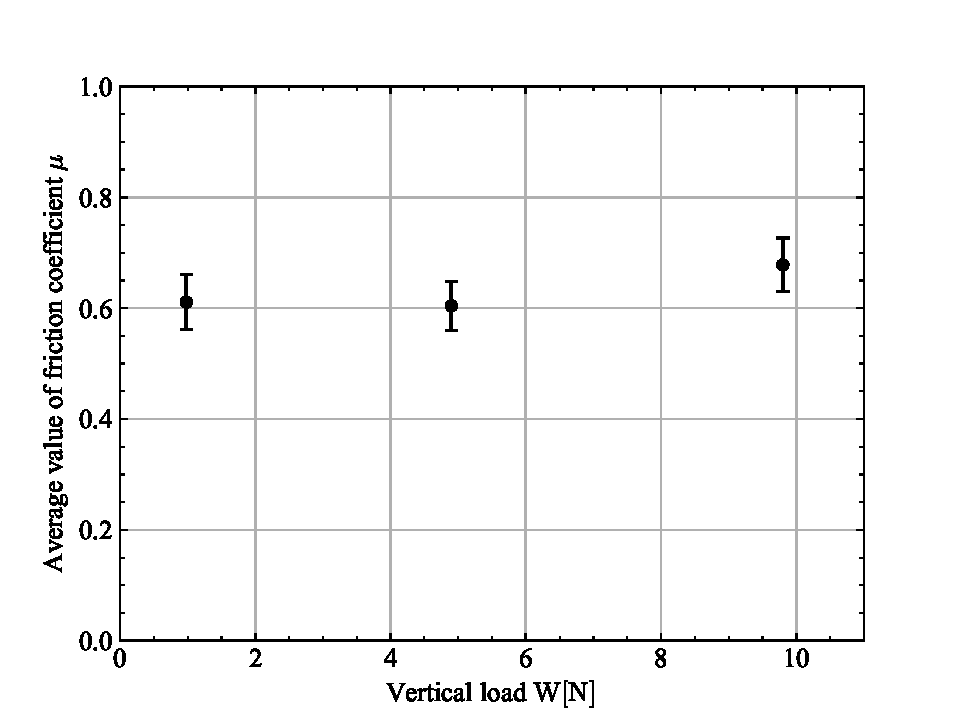
\includegraphics[width=100truemm,clip]{fig/fig_1mm.pdf}
    \caption{Value of coefficient of friction for vertical load(R=1[mm]).}
    \label{fig:fig_1mm}
\end{figure}

\begin{figure}[htbp]
    \centering %中央揃え
    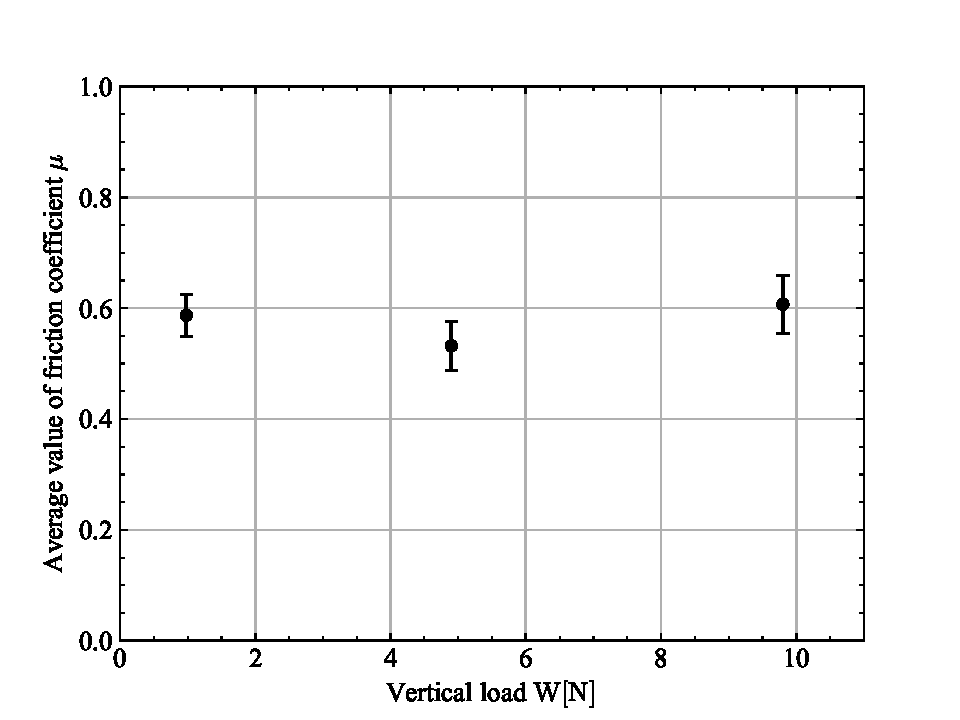
\includegraphics[width=100truemm,clip]{fig/fig_4mm.pdf}
    \caption{Value of coefficient of friction for vertical load(R=4[mm]).}
    \label{fig:fig_4mm}
\end{figure}
\clearpage
\begin{figure}[htbp]
    \centering %中央揃え
    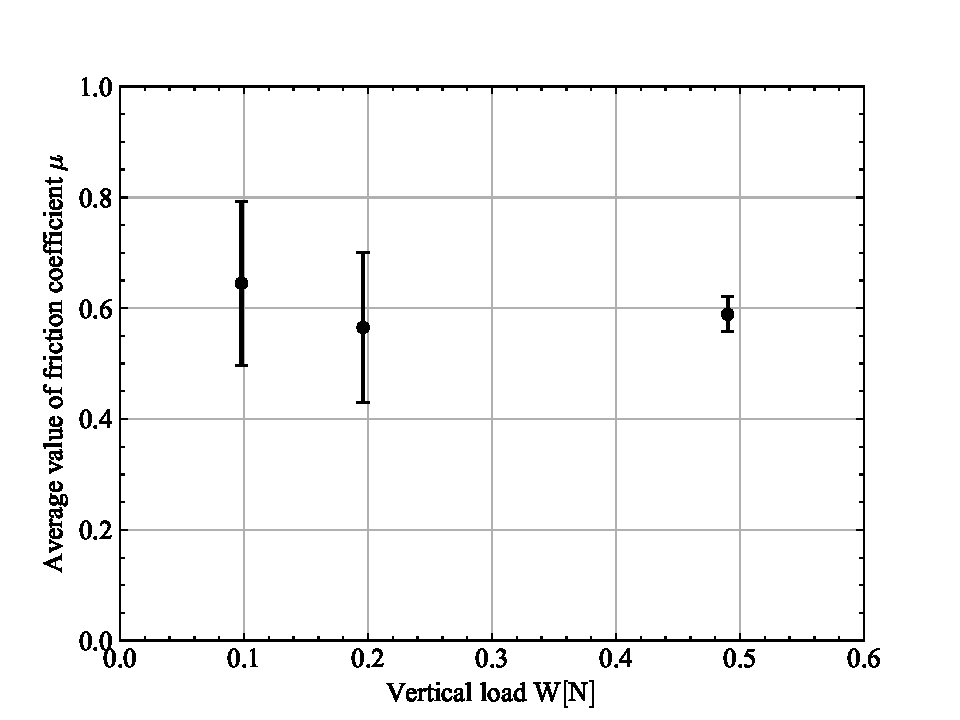
\includegraphics[width=100truemm,clip]{fig/fig_8mm.pdf}
    \caption{Value of coefficient of friction for vertical load(R=8[mm]).}
    \label{fig:fig_8mm}
\end{figure}

\subsection{$\mathrm{P_m/H_v}$値および静的接触形態について}
ヘルツの弾性接触理論を用いて,各摩擦条件における理論上の接触面積$A$,平均接
触圧力$P_m$,$\mathrm{P_m/H_v}$値および静的接触形態を表\ref{tbl:平均圧力1mm}から表\ref{tbl:平均圧力8mm}にかけて示す.

$\mathrm{P_m/H_v}$値を横軸,摩擦係数$\mu$を縦軸としてプロットしたものを図\ref{fig:fig_Pm}に示す.$\mathrm{P_m/H_v}$値の変化による摩擦係数の大きな変化は見られなかった.しかし,おおよその傾向として$\mathrm{P_m/H_v}$ = 0から0.5付近の範囲では値の増加に伴って摩擦係数がやや減少.$\mathrm{P_m/H_v}$ = 0.6から1.3付近の範囲ではは摩擦係数0.6まで増加してほぼ一定の値となり,$\mathrm{P_m/H_v}$ = 1.7で再び増加するグラフとなっている.

\begin{table}[htbp]
    \centering
    \caption{Theoretical contact area, average contact pressure, $\mathrm{P_m/H_v}$ value and static contact morphology(R=1[mm]).}
    \label{tbl:平均圧力1mm}
    \scalebox{1.0}{
    \begin{tabular}{cccc}
    \hline
    垂直荷重 {[}N{]}    & 0.98    & 4.9     & 9.8     \\ \hline
    接触円半径{[}mm{]}   & 0.0234  & 0.0400  & 0.0504  \\ \hline
    接触円面積{[}mm2{]}  & 0.00172 & 0.00503 & 0.00798 \\ \hline
    平均接触圧力{[}GPa{]} & 0.570   & 0.975   & 1.23    \\ \hline
    Pm/Hv           & 0.771   & 1.318   & 1.66    \\ \hline
    静的接触形態          & 弾塑性接触   & 塑性接触    & 塑性接触    \\ \hline
    \end{tabular}
    }
\end{table}

\begin{table}[htbp]
    \centering
    \caption{Theoretical contact area, average contact pressure, $\mathrm{P_m/H_v}$ value and static contact morphology(R=4[mm]).}
    \label{tbl:平均圧力4mm}
    \scalebox{1.0}{
    \begin{tabular}{cccc}
    \hline
    垂直荷重 {[}N{]}    & 0.98    & 4.9    & 9.8    \\ \hline
    接触円半径{[}mm{]}   & 0.0371  & 0.0635 & 0.0800 \\ \hline
    接触円面積{[}mm2{]}  & 0.00433 & 0.0127 & 0.0201 \\ \hline
    平均接触圧力{[}GPa{]} & 0.226   & 0.387  & 0.488  \\ \hline
    Pm/Hv           & 0.306   & 0.523  & 0.659  \\ \hline
    静的接触形態          & 弾性接触    & 弾塑性接触  & 弾塑性接触  \\ \hline
    \end{tabular}
    }
\end{table}

\begin{table}[htbp]
    \centering
    \caption{Theoretical contact area, average contact pressure, $\mathrm{P_m/H_v}$ value and static contact morphology(R=8[mm]).}
    \label{tbl:平均圧力8mm}
    \scalebox{1.0}{
    \begin{tabular}{cccc}
    \hline
    垂直荷重 {[}N{]}    & 0.098   & 0.196   & 0.49    \\ \hline
    接触円半径{[}mm{]}   & 0.0217  & 0.0274  & 0.0371  \\ \hline
    接触円面積{[}mm2{]}  & 0.00148 & 0.00235 & 0.00433 \\ \hline
    平均接触圧力{[}GPa{]} & 0.0662  & 0.0834  & 0.1132  \\ \hline
    Pm/Hv           & 0.0894  & 0.113   & 0.153   \\ \hline
    静的接触形態          & 弾性接触    & 弾性接触    & 弾性接触    \\ \hline
    \end{tabular}
    }
\end{table}

\begin{figure}[htbp]
    \centering %中央揃え
    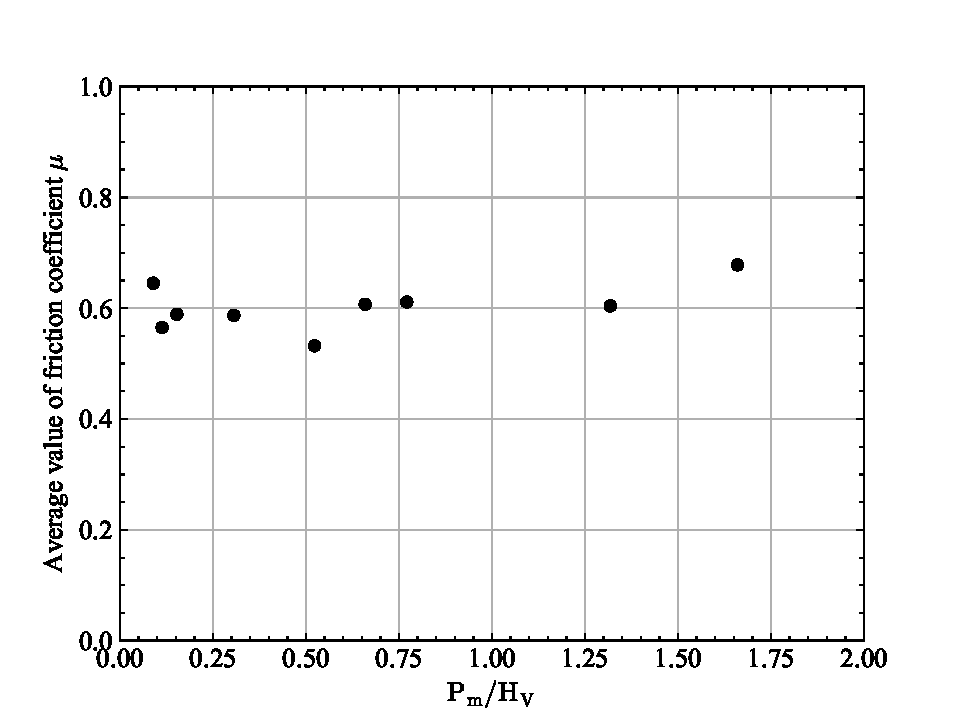
\includegraphics[width=100truemm,clip]{fig/fig_PmHv.pdf}
    \caption{Relationship between coefficient of friction and $\mathrm{P_m/H_v}$ value.}
    \label{fig:fig_Pm}
\end{figure}

